\documentclass{article}
\usepackage[portuguese]{babel}
\usepackage{graphicx}
\usepackage{listings}
\usepackage[utf8]{inputenc}
\usepackage{listings}
%\graphicspath{ {/home/jessica/Documentos/Engineer/Geocaching-Java} }

\renewcommand{\baselinestretch}{2}
%\author{no realizado por :P}
\title{Geocaching POO}
\date{Junho 2015}
\begin{document}
\maketitle
\begin{center}
Realizado por: \\
Jéssica Pereira a71164	\\
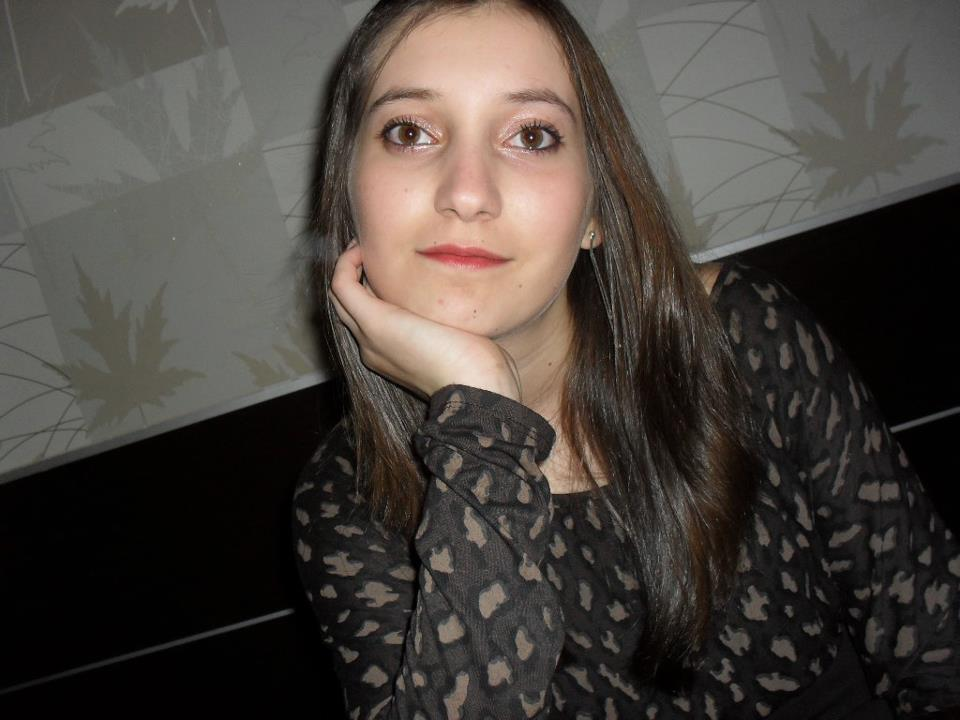
\includegraphics[height=3\baselineskip,natwidth=369,natheight=430]{jessica0.jpg}\\
Adelino Costa a70563\\
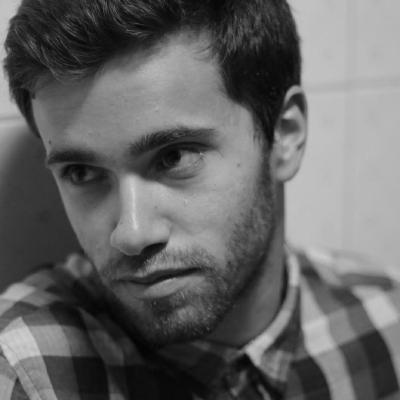
\includegraphics[height=3\baselineskip,natwidth=369,natheight=430]{adelino.jpg}\\
Martinho Aragão a72205 \\

\includegraphics[height=3\baselineskip,natwidth=369,natheight=430]{martinho.jpg}
\end{center}

\pagebreak


\tableofcontents

\pagebreak

\section{Introdução}

\quad
Este trabalho sobre o conceito de Geocaching conhecido nas redes sociais: pretendemos simular
e registar atividades e descobrimentos de caches. Para isso foi necessário modularizar e fazer
as devidas abstrações na preparação para o trabalho, pois quanto mais abstrações forem criadas
mais independentes os módulos serão, podendo depois usar a composição entre estas classes e
fornecendo uma melhor compreensão do código e tratamento da informação.
\par
É necessário o estudo e concepção das classes necessárias, estruturas de dados, métodos
respetivos, variáveis de instância e de classe necessárias, imagina a dependência entre
as classes (composição) e definir uma hierarquia (nomeadamente criando uma super
class para as Caches).
\par Para além de criar classes abstratas, também é necessário guardar todos os dados relativos
às Caches e aos Utilizadores para poder criar métodos eficientes relativos ao tratamento
destes.
\par De entre os requesitos básicos também serão implementados os Eventos, com a simulação
da metereologia e cálculo de distâncias entre caches dados duas coordenadas (coordenadas
iniciais e as coordenadas da cache). Estes dois últimos pontos serão implementados também
em toda a descoberta de Caches/Actividades e não somente no decorrer de Eventos pois serão
úteis nomeadamente para o cálculo de pontuações.
\pagebreak

%Na introdução foram ditos os objetivos. :P

\section{Modularização - Classes criadas}

%adicionar imagem do trello final do diagrama

\pagebreak
\section{Bases de dados}

\subsection{CacheBase}
\par Antes de implementarmos a classe \textbf{CacheBase} reflectimos que características únicas teria cada cache para a 
diferenciar de todas as outras.
\par Cada cache tem coordenadas únicas, não sendo possível criar uma cache em coordenadas onde já existe uma cache, 
independentemente do tipo de cache, isto levou-nos a implementar um \textbf{TreeMap} para mapear coordenadas a 
IDs de cache.
\par Para guardar as caches utilizamos um \textbf{ArrayList} visto que sabendo o ID de uma cache é bastante fácil encontrá-lo 
nesta estrutura pois para um dado valor de ID sabemos que a Cache, caso exista, estará no indíce de valor igual a (ID - 1).
\par Portanto a implementação das variáveis de instância de \textbf{CacheBase} é a seguinte:
\begin{lstlisting}[language=Java]
/* ArrayList com as caches */
private ArrayList<Cache> caches;
/* Mapeamento entre e-mails e IDs */
private TreeMap<Coordinates, Double> coords;
\end{lstlisting}

\par Como é necessário um dado Utilizador poder ver as caches que criou utilizamos um \textbf{TreeMap} para mapear 
IDs de Utilizadores a um \textbf{ArrayList} que contém os IDs das caches que o Utilizador criou, caso tenha criado alguma.
\begin{lstlisting}[language=Java]
/* Mapeamento IDs de Utilizadores e IDs de Caches */
private TreeMap<Double, ArrayList<Double>> owners;
\end{lstlisting}

\par Finalmente para implementar o 'report' de Caches criámos outra variável de instância que mapea-se IDs de Caches 
a \textbf{ArrayList} de Reports dessa Cache.
\begin{lstlisting}[language=Java]
/* Mapeamento entre IDs de Caches e Reports dessa cache */
private TreeMap<Double, ArrayList<Report>> reported_caches;
\end{lstlisting}

\newpage
\subsection{UserBase}
\par Para guardar tanto Utilizadores como Administratores primeiros pensamos nas várias maneiras de referenciar um 
Utilizador, assumimos que as maneiras de referenciar um Utilizador seria através do seu ID ou através do seu e-mail.
\par Para os Utilizadores criámos utilizamos um \textbf{TreeMap} que faz o mapeamento de um e-mail para um ID, e 
utilizamos um \textbf{ArrayList} para guardar os Utilizadores pois torna-se bastante rápido encontrar um utilizador dado o
seu ID, visto que para um dado ID o Utilizador, caso exista, estará no indice de valor igual a (ID - 1) no \textbf{ArrayList}.
\par Ficaram então definidas desta forma as variáveis de instância de \textbf{UserBase}:
\begin{lstlisting}[language=Java]
/* ArrayList com os utilizadores */
private ArrayList<NormalUser> users;
/* Mapeamento entre e-mails e IDs */
private TreeMap<String, Double> userMails;
\end{lstlisting}

\par Para guardar as várias instâncias de \textbf{Admin} utilizamos o mesmo método que no caso das instâncias de
\textbf{NormalUser}. Segue-se a definição das variáveis de instância:
\begin{lstlisting}[language=Java]
/* ArrayList com os administradores */
private ArrayList<Admin> admins;
/* Mapeamento entre e-mails e IDs */
private TreeMap<String, Double> adminMails;
\end{lstlisting}

\pagebreak
\section{Programa Principal e Main}
\quad Na classe \textbf{GeocachingPOO} estão as chamadas de todos os métodos existentes em todas as classes que 
permitem uma interação a nível de Objetos.

\par No Main estão todos os Menus e toda a interação I/O entre o utilizador e o nosso programa.Com isto permitimos que o nosso programa possa ser implementado com outras Interfaces Gráficas, nomeadamente para a web, etc. ...

\pagebreak
\section{Tratamento de Excepções}
\quad Decidimos colocar todas as excepções num package chamado Exceptions para uma melhor visualização das classes e 
clareza no diagrama. Para todas as classes que implementam Excepções é feito import deste Package. Apenas a função 
\em main faz o tratamento de Excepções.
\pagebreak
\section{Conclusão}



\pagebreak
\section{}
\subsection{}
\subsubsection{}

\paragraph{paragraph title here}


\end{document}